\section{Linear Maps}

  Remember that a linear transformation is just a homomorphism between vector spaces. That is, given linear transformation $T: U \longrightarrow V$, 
  \begin{equation}
    T \in \text{Hom}(U,V)
  \end{equation}

  \begin{figure}[H]
    \centering 
    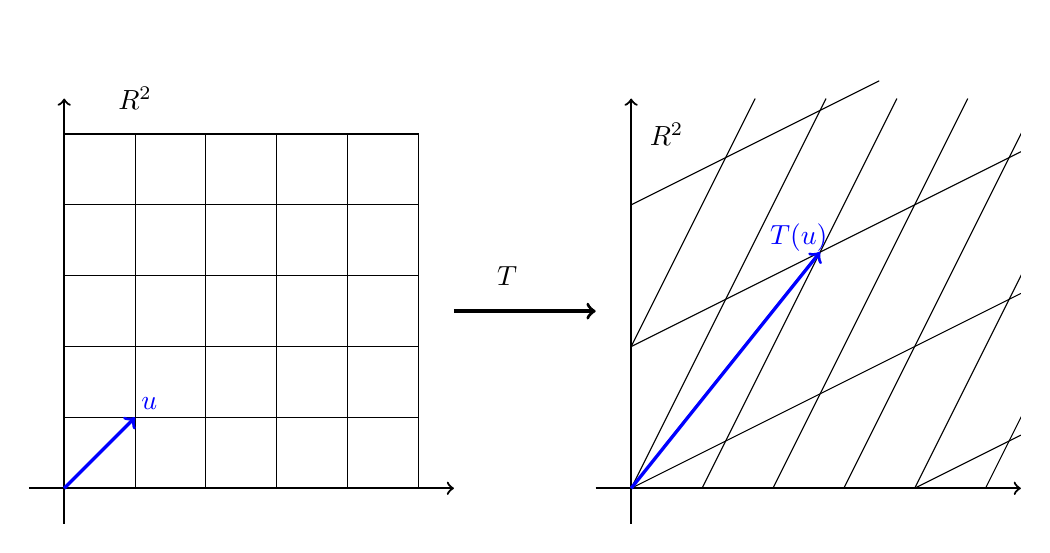
\begin{tikzpicture}[scale=0.9]
      % Left grid (domain)
      \begin{scope}[shift={(-5,0)}]
        % Draw grid
        \draw[step=1cm, black] (0,0) grid (5,5);
        
        % Draw axes
        \draw[thick, ->] (-0.5,0) -- (5.5,0);
        \draw[thick, ->] (0,-0.5) -- (0,5.5);
        
        % Label the space
        \node at (1,5.5) {$\mathbb{R}^2$};
        \draw[->, very thick, blue] (0, 0) -- (1, 1);
        \node[blue] at (1.2,1.2) {$u$};
      \end{scope}
      
      % Transformation arrow
      \draw[->, very thick] (0.5,2.5) -- (2.5,2.5);
      \node at (1.25,3) {$T$};

      
      % Right grid (codomain)
      \begin{scope}[shift={(3,0)}]
        % Draw only axes
        \draw[thick, ->] (-0.5,0) -- (5.5,0);
        \draw[thick, ->] (0,-0.5) -- (0,5.5);
        
        % Label the space
        \node at (0.5,5) {$\mathbb{R}^2$};
        
        % Clip all drawing to stay within visible area
        \begin{scope}
          \clip (-0.5,-0.5) rectangle (5.5,6.5);
          
          % Existing lines with slope 1/2
          \draw[] (4,0) -- (5.5,0.75);
          \draw[] (0,0) -- (5.5,2.75);
          \draw[] (0,2) -- (5.5,4.75);
          \draw[] (0,4) -- (3.5,5.75);
          
          % New lines with slope 2
          \draw[] (5,0) -- (7.75,5.5);
          \draw[] (4,0) -- (6.75,5.5);
          \draw[] (3,0) -- (5.75,5.5);
          \draw[] (2,0) -- (4.75,5.5);
          \draw[] (1,0) -- (3.75,5.5); 
          \draw[] (0,0) -- (2.75,5.5); 
          \draw[] (0,2) -- (1.75,5.5); 
        \end{scope}
        \node[blue] at (2.366,3.533) {$T(u)$};
        \draw[->, very thick, blue] (0, 0) -- (2.666, 3.333);
      \end{scope}
    \end{tikzpicture}
    \caption{We can visualize all linear transformations as "transforming" the axes as shown below. }
    \label{fig:linear_map}
  \end{figure}

  \begin{definition}[Image]
    The \textbf{image}, or \textbf{range} of $T: U \longrightarrow V$ is the image of $U$ under $T$, denoted Im$T$. 
    \begin{equation}
      \im{T} \equiv \{ T(u) \; | \; u \in U\} \subset V
    \end{equation}
    The \textbf{kernel or nullspace} of $T$ is the subset of $U$ that is mapped onto $0$, denoted ker$T$. 
    \begin{equation}
      \text{ker}\,T \equiv \{ u \in U \; | \; T(u) = 0\}
    \end{equation}
  \end{definition}

  \begin{example}
    Let $U_1$ be a subspace of $U$ and given the quotient map
    \begin{equation}
      \pi: U \longrightarrow U / U_1
    \end{equation}
    Then, 
    \begin{equation}
      \text{ker}\,\pi = U_1, \; \im{\pi} = U / U_1
    \end{equation}
    Note that a quotient map is always surjective. 
  \end{example}

  \begin{theorem}[Rank Nullity Theorem]
    Let $T: U \longrightarrow V$ be linear. Then, 
    \begin{equation}
      \dim \ker T + \dim \im T = \dim U
    \end{equation}
    This theorem is quite intuitive, if we visualize the map. 

    \begin{figure}[H]
      \centering 
      \begin{tikzpicture}
        % Add R³ label for the left side
        \node at (-2.9,2.1) {$\mathbb{R}^3$};
        
        % Add R² label for the right side
        \node at (2,2.1) {$\mathbb{R}^2$};
        
        % Left diagram - Parallelogram with kernel
        \begin{scope}[shift={(-4,0)}]
          % Rotate the entire picture 30 degrees clockwise
          \begin{scope}[rotate=-30]
            % Define coordinates for the parallelogram
            \coordinate (A) at (-2,-1);
            \coordinate (B) at (2,-1);
            \coordinate (C) at (1,1);
            \coordinate (D) at (-3,1);
            
            % Draw the parallelogram with red fill
            \fill[red, opacity=0.3] (A) -- (B) -- (C) -- (D) -- cycle;
            \draw (A) -- (B) -- (C) -- (D) -- cycle;
            
            % Draw the dashed portion where the line intersects the parallelogram in blue
            \draw[dashed, thick, blue] (-0.5,-2) -- (-0.5,2);
            
            % Add a dot at intersection point
            \filldraw (-0.5,0) circle (2pt);
            
            % Label the dashed line in blue
            \node[blue] at (0.8,0) {$\mathrm{ker}(T)$};
          \end{scope}
        \end{scope}
        
        % Arrow connecting the two diagrams
        \draw[-{Stealth[length=3mm,width=2mm]}] (-1,0) -- (1,0);
        \node at (0,0.5) {$T$};
        
        % Right diagram - Real plane
        \begin{scope}[shift={(4,0)}]
          % Fill the background with red
          \fill[red, opacity=0.3] (-2.5,-2.5) rectangle (2.5,2.5);
          
          % Draw the x and y axes
          \draw[->] (-2.2,0) -- (2.2,0) node[right] {$x$};
          \draw[->] (0,-2.2) -- (0,2.2) node[above] {$y$};
          
          % Add tick marks
          \foreach \x in {-2,-1,1,2}
            \draw (\x,0.1) -- (\x,-0.1) node[below] {$\x$};
          \foreach \y in {-2,-1,1,2}
            \draw (0.1,\y) -- (-0.1,\y) node[left] {$\y$};
          
          % Mark the origin with a blue point
          \filldraw[blue] (0,0) circle (2.5pt);
        \end{scope}
      \end{tikzpicture}
      \caption{We just have to realize that given a linear transformation mapping from a $n$-dimensional $V$ to a $m$-dimensional $U$, every vector in $V$ will either get mapped to $0 \in U$ or will get mapped to a nonzero vector in $U$. In this case, the kernel will get mapped to $0$ and everything else is (not always, but in this case) $\mathbb{R}^2$. } 
      \label{fig:rank_nullity}
    \end{figure}
  \end{theorem}

  \begin{proposition}
    Hom$(U, V)$ is the vector space of linear mappings, with addition and scalar multiplication defined
    \begin{align*}
      & (S + T) (x) \equiv S(x) + T(x) \\
      & (c T) (x) \equiv c T(x)
    \end{align*}
  \end{proposition}

  \begin{definition}[Composition]
    The \textbf{composition} of linear functions, denoted with $\circ$, is defined
    \begin{equation}
      (S \circ T) (x) \equiv S\big( T(x)\big)
    \end{equation}
    Given $T \in $ Hom$(U, V)$ and $S \in $ Hom$(V, W)$, then $S \circ T \in $ Hom$(U, W)$. For simplicity, we also denote the composition as 
    \begin{equation}
      S \circ T \equiv S T
    \end{equation}
  \end{definition}

  \begin{proposition}[Composition is Distributive]
    Composition is (right and left) distributive with respect to the addition of linear maps. That is, 
    \begin{align*}
      & (R + S) \circ T = R \circ T + S \circ T \\
      & T \circ (R + S) = T \circ R + T \circ S 
    \end{align*}
  \end{proposition}

  \begin{definition}[Algebra]
    An \textbf{algebra} $A$ is a vector space with the additional operation of vector multiplication. That is, $A$ is closed under 
    \begin{equation}
      \circ: A \times A \longrightarrow A
    \end{equation}
    An algebra is \textbf{associative} if multiplication is associative. That is, given $R, S, T \in A$
    \begin{equation}
      R \circ (S \circ T) = (R \circ S) \circ T
    \end{equation}
    Note that multiplication is not necessarily commutative. 
  \end{definition}

  \begin{proposition}
    End$(V)$ is an associative, noncommutative algebra. 
  \end{proposition}

  \begin{example}
    A rotation around any axis or a flip across any hyperplane is an element of End$(\mathbb{R}^n)$. 
  \end{example}

  \begin{definition}[Projection]
    A \textbf{projection mapping} is a linear mapping $P$ where 
    \begin{equation}
      P = P^2
    \end{equation}
  \end{definition}

  \begin{example}
    Let $P$ be an orthogonal projection mapping onto a subspace $Y$ of $X$. $\im P = Y$, and $\ker P = Y^\perp$ or the span of vectors in $X$ that are "orthogonal" to $Y$. Note that we haven't actually endowed a structure onto $X$ to even define orthogonality yet, so this definition is purely visual and not mathematically rigorous. 
  \end{example}

  \begin{example}
    Reflections, projections, shears, and rotations are all linear maps. Differentiation and integration are also examples of linear mappings. 
  \end{example}

  Linear maps over vector spaces over different fields are generally not well defined since the definition of homomorphisms do not cover the fields in which vector spaces are associated with. 

  \begin{theorem}
    Given $A: V \longrightarrow U$ a linear mapping between vector spaces and $b \in U$, all solutions to the equation $Ax = b$ is in $a + \ker A$, that is, of the form 
    \begin{equation}
      x = a + y, \; y \in \ker A
    \end{equation}
    where $x = a$ is one solution. 
  \end{theorem}

  \begin{corollary}
    A linear map $A$ is injective if and only if $\ker A = 0$.
  \end{corollary}

  \begin{definition}[Rank]
    The \textbf{rank} of a linear map $A$ is the dimension of its image. 
  \end{definition}

\subsection{Factorization of Linear Maps}

  \begin{definition}[Restriction]
    Let $\varphi: U \longrightarrow V$ be a linear mapping and let $U_1 \subset U, V_1 \subset V$ be subspaces. Such that 
    \begin{equation}
      \varphi u \in V \text{ for all } u \in U
    \end{equation}
    Then, the linear mapping 
    \begin{equation}
      \varphi_1: U_1 \longrightarrow V_1, \; \varphi_1 u = \varphi_u, u \in U_1
    \end{equation}
    is called the \textbf{restriction} of $\varphi$ to $U_1, V_1$. It suffices the identity
    \begin{equation}
      \varphi \circ i_U = i_V \circ \varphi_1
    \end{equation}
    where $i_U: U_1 \longrightarrow U, i_V: V_1 \longrightarrow V$ are canonical injections. Equivalently, we say that the diagram below is \textbf{commutative}. 
    \[
      \begin{tikzcd}
        U \arrow{r}{\varphi} & V \\
        U_1 \arrow{u}{i_U} \arrow{r}{\varphi_1} & V_1 \arrow{u}{i_V}
      \end{tikzcd}
    \]
    We can also define 
    \begin{equation}
      \varphi_1 \equiv i_v^{-1} \varphi i_U
    \end{equation}
  \end{definition}

  The construction of the restriction is an enormously helpful tool for many proofs and very useful for factoring linear mappings. 

  \begin{definition}[Induced Mapping of Quotients]
    Given $\varphi: U \longrightarrow V$ with quotient maps 
    \begin{equation}
      \pi_U: U \longrightarrow U / U_1, \; \pi_V: V \longrightarrow V / V_1
    \end{equation}
    the \textbf{induced mapping of the quotient spaces} is the unique mapping $\bar{\varphi}: U/U_1 \longrightarrow V / V_1$ such that 
    \begin{equation}
      \bar{\varphi} \circ \pi_U = \pi_V \circ \varphi
    \end{equation}
    or equivalently, the following diagram commutes. 
    \[\begin{tikzcd}
        U \arrow{r}{\varphi} \arrow{d}{\pi_U} & V \arrow{d}{\pi_V}\\
        U / U_1 \arrow{r}{\bar{\varphi}} & F / F_1
    \end{tikzcd}\]
  \end{definition} 

  \begin{theorem}
    Every linear mapping can be written as the composition of a surjective mapping followed by an injective mapping. That is, every $A$ can be factored into 
    \begin{equation}
      A = A_{inj} \circ A_{surj}
    \end{equation}
  \end{theorem}
  \begin{proof}
    We can induce a quotient mapping to construct a factoring of a linear mapping. We can define the unique mapping 
    \begin{equation}
      \bar{\varphi}: U / \ker{U} \longrightarrow F
    \end{equation}
    such that, $\varphi = \bar{\varphi} \circ \pi_U$, or that 
    \[\begin{tikzcd}
       U \arrow{r}{\varphi} \arrow{d}{\pi_U} & V \\
       U / \ker{\varphi} \arrow{ru}{\bar{\varphi}}
    \end{tikzcd} \]
    commutes. Clearly, $\bar{\varphi}$ is injective since if it were not, $\bar{\varphi} \pi_U x = 0 \implies \varphi x = 0 \implies x \in \ker{\varphi} \implies \pi_U x = 0$. This also means that the restriction of $\bar{\varphi}$ to $U / \ker{\varphi}$
    \begin{equation}
      \bar{\bar{\varphi}}: U / \ker{\varphi} \longrightarrow \im{\varphi}
    \end{equation}
    is a linear isomorphism. Thus, for any $\varphi$, it can be written as $\bar{\varphi} \circ \pi_U$, with $\bar{\varphi}$ injective and $\pi_U$ surjective. 
  \end{proof}

  \begin{proposition}
    Given $E_1, E_2$ subspaces of $E$. Then, 
    \begin{equation}
      \frac{E_1}{E_1 \cap E_2} \simeq \frac{E_1 + E_2}{E_2}
    \end{equation}
    In fact, they are naturally isomorphic. 
  \end{proposition}
  \begin{proof}
    $E_1 + E_2$ can be decomposed to $E_1^\prime \oplus (E_1 \cap E_2) \oplus E_2^\prime$, where $E_1^\prime$ consists of the subspace of vectors $x$ that can only be expressed as $x = x_1, x_1 \in E_1$ and $E_2^\prime$ are vectors that can only be expressed as $x = x_2, x_2 \in E_2$. Define the projection mapping
    \begin{equation}
      \text{proj}: E_1 + E_2 \longrightarrow E_1^\prime
    \end{equation}
    Since $E_1 = E_1^\prime \oplus (E_1 \cap E_2)$, we can define the natural isomorphism 
    \begin{equation}
      \kappa: E_1^\prime \longrightarrow \frac{E_1}{E_1 \cap E_2}, \; \kappa{x} = \{x\}
    \end{equation}
    We now define the mapping $\varphi: E_1^\prime \longrightarrow (E_1 + E_2) / E_2$ such that
    \begin{equation}
      \pi = \varphi \text{proj}
    \end{equation}
    given by the diagram 
    \[\begin{tikzcd} 
        E_1 + E_2 \arrow{d}{proj} \arrow{r}{\pi} & \frac{E_1 + E_2}{E_2} \\
        E_1^\prime \arrow{ru}{\varphi} \arrow{r}{\kappa} & \frac{E_1}{E_1 \cap E_2}
    \end{tikzcd}\]
    Such a $\varphi$ exists because proj is surjective and can thus be inverted. We now claim that $\varphi$ is an isomorphism. $\ker{\text{proj}} = \ker{\pi} = E_2 \implies \kappa$ is injective. Given $x = x_1 + y + x_2 \in E_1 + E_2$ such that $x_1 \in E_1^\prime, y \in E_1 \cap E_2, x_2 \in E_2^\prime$, 
    \begin{equation}
      \pi(x) = \pi(x_1 + y + x_2) = \pi(x_1) = \varphi \text{proj} (x_1) = \varphi (x_1)
    \end{equation}
    meaning that for every vector $v \in (E_1 + E_2) / E_2$, it can be expressed as $v = \pi (x) = \varphi (x_1)$, meaning that there exists a $x_1 \in E_1^\prime$ mapping to $v$ under $\varphi \iff \varphi$ is surjective. So, $\varphi$ is an isomorphism $\implies \varphi \kappa^{-1}$ is an isomorphism.  
  \end{proof}

  \begin{corollary}
    In the special case when $E_1 \oplus E_2 = E$, then the proposition states that 
    \begin{equation}
      E_1 \simeq \frac{E}{E_2}
    \end{equation}
  \end{corollary}

  Let $f_1, f_2, ..., f_n$ be any $n$ linear functionals of $U$. Define the subspace $F \subset E$ as 
  \begin{equation}
    F \equiv \bigcap_{i=1}^n \ker{f_i}
  \end{equation}
  and define linear map 
  \begin{equation}
    \phi: U \longrightarrow \mathbb{F}^n, \;\phi(x) \equiv (f_1(x), f_2(x), ..., f_n(x))
  \end{equation}
  $\implies \ker{\phi} = F$. So, $\phi: U \longrightarrow \mathbb{F}^n$ defines the isomorphism 
  \begin{equation}
    \bar{\phi}: U / F \longrightarrow \im{\phi}
  \end{equation}

  \begin{proposition}
    Given linear mappings $\phi: E \longrightarrow F$, $\psi: E \longrightarrow G$ such that
    \begin{equation}
      \ker{\phi} \subseteq \ker{\psi}
    \end{equation}
    Then there exists a map $\kappa$ such that 
    \begin{equation}
      \psi = \kappa \phi
    \end{equation}
    or equivalently, such that the diagram below commutes. 
    \[\begin{tikzcd} 
        E \arrow{r}{\phi} \arrow{d}{\psi} & F \arrow{dl}{\kappa} \\
        G 
    \end{tikzcd}\]
  \end{proposition}

  Now, we introduce the concept of exact sequences which is useful in the factoring of linear maps. Note that exact sequences are used in group theory to factor transformation groups. 

  \begin{definition}
    A sequence of linear mappings 
    \begin{equation}
      F \xrightarrow{\varphi} E \xrightarrow{\psi} G
    \end{equation}
    is \textbf{exact at E} if
    \begin{equation}
      \im{\varphi} = \ker{\psi}
    \end{equation}
  \end{definition}

  Notice that if we have an exact sequence 
  \begin{equation}
    0 \xrightarrow{\varphi} E \xrightarrow{\psi} G
  \end{equation}
  then, $0 = \im{\varphi} = \ker{\psi} \implies \psi$ is injective. If we have exact sequence 
  \begin{equation}
    F \xrightarrow{\varphi} E \xrightarrow{\psi} 0
  \end{equation}
  then, $\im{\varphi} = \ker{\psi} = E \implies \varphi$ is surjective. 

  \begin{definition}
    A \textbf{short exact sequence} is a sequence of the form
    \begin{equation}
      0 \xrightarrow{} F \xrightarrow{\varphi} E \xrightarrow{\psi} G \xrightarrow{} 0
    \end{equation}
    such that it is exact at $F, E$, and $G$. It is clear that the first and last maps are the zero maps. With this definition, we can easily prove that
    \begin{enumerate}
      \item $\varphi$ is injective
      \item $\psi$ is surjective
      \item $E / \im{F} \simeq G$
    \end{enumerate}
  \end{definition}

  \begin{example}
    The sequence 
    \begin{equation}
      0 \xrightarrow{} E_1 \xrightarrow{i} E \xrightarrow{\pi} E / E_1 \xrightarrow{} 0
    \end{equation}
    is exact, where $i$ denotes the canonical injection and $\pi$ the canonical projection. This example is the only example of an exact sequence between vector spaces up to isomorphism. 
  \end{example}

  \begin{definition}
    A commutative diagram of the form
    \[\begin{tikzcd}
        0 \arrow{r} & F_1 \arrow{d}{\alpha} \arrow{r}{\varphi_1} & E_1 \arrow{d}{\beta} \arrow{r}{\psi_1} & G_1 \arrow{d}{\gamma} \arrow{r} & 0 \\
        0 \arrow{r} & F_2 \arrow{r}{\varphi_2} & E_2 \arrow{r}{\psi_2} & G_2 \arrow{r} & 0 
    \end{tikzcd}\]
    where both horizontal sequences are short exact sequences and $\alpha, \beta, \gamma$ are homomorphisms between linear spaces is a \textbf{homomorphism of exact sequences}. If $\alpha, \beta, \gamma$ are linear isomorphisms, then this is an \textbf{isomorphism of exact sequences}. 
  \end{definition}

  \begin{proposition}
    A short exact sequence of vector spaces
    \begin{equation}
      0 \xrightarrow{} F \xrightarrow{\varphi} E \xrightarrow{\psi} G \xrightarrow{} 0
    \end{equation}
    is split if it essentially presents $E$ as the direct sum of groups $F$ and $G$. That is, there exists an isomorphism of exact sequences.
    \[\begin{tikzcd}
        0 \arrow{r} & F \arrow{d}{\alpha} \arrow{r}{\varphi_1} & E \arrow{d}{\beta} \arrow{r}{\psi_1} & G \arrow{d}{\gamma} \arrow{r} & 0 \\
        0 \arrow{r} & F \arrow{r}{\varphi_2} & F \oplus G \arrow{r}{\psi_2} & G \arrow{r} & 0 
    \end{tikzcd}\]
    or equivalently, there exists an isomorphism between $E$ and $F \oplus G$. 
  \end{proposition}

  \begin{definition}
    Given a short exact sequence
    \begin{equation}
      0 \xrightarrow{} F \xrightarrow{\varphi} E \xrightarrow{\psi} G \xrightarrow{} 0
    \end{equation}
    if there exists a map $\kappa: G \longrightarrow E$, such that $ \psi \circ \kappa = I$, then the sequence is said to be a \textbf{split short exact sequence}, written
    \begin{equation}
      0 \xrightarrow{} F \xrightarrow{\varphi} E \xleftrightarrow{\psi, \kappa} G \xrightarrow{} 0
    \end{equation}
  \end{definition}

  \begin{proposition}
    Every short exact sequence can be split. 
  \end{proposition}
  \begin{proof}
    It will be proved later that $\psi$ is surjective $\implies$ $\psi$ is left invertible. 
  \end{proof}

  \begin{definition}[Stable Subspaces]
    Given $\varphi: E \longrightarrow E$, a subspace $E_1 \subset E$ is called \textbf{stable} 
    \begin{equation}
      x \in E_1 \implies \varphi x \in E_1
    \end{equation}
    That is, the restriction of $\varphi$ to $E_1$, denoted
    \begin{equation}
      \varphi: E_1 \longrightarrow E_1
    \end{equation}
    is well-defined. Clearly, $\im{\varphi}$ and $\ker{\varphi}$ is stable, and the induced map 
    \begin{equation}
      \bar{\varphi}: E / E_1 \longrightarrow E / E_1
    \end{equation}
    is a linear endomorphism of $E / E_1$. 
  \end{definition}

  We end this subsection by defining the induced linear map from the direct sum of spaces. 

  \begin{definition}
    Given linear maps $A_i \in$ End$(V_i)$ for $i = 1, 2, ..., n$, the induced linear map
    \begin{equation}
      \bigoplus_{i =1}^n A_i: \bigoplus_{i=1}^n V_i \longrightarrow \bigoplus_{i=1}^n V_i
    \end{equation}
    is defined
    \begin{equation}
      (\bigoplus_{i=1}^n A_i)(\bigoplus_{i=1}^n x_i) \equiv \bigoplus_{i=1}^n A_i x_i
    \end{equation}
  \end{definition}

\subsection{Invertibility and Transpose}

  We now introduce the concepts of left and right invertibility of linear mappings. 

  \begin{theorem}[Left/Right-Invertibility]
    A linear mapping $T: U \longrightarrow V$, with $\dim{U} = n, \dim{V} = m$, is \textbf{left-invertible}. That is, there exists linear $S$ such that 
    \begin{equation}
      S T = I
    \end{equation}
    if and only if $T$ is injective $\iff$ rank$(T) = n$. Linear $T$ is \textbf{right-invertible}, that is, there exists linear $S$ such that 
    \begin{equation}
      T S = I
    \end{equation}
    if and only if $T$ is surjective $\iff$ rank$(T) = m$. 
  \end{theorem}
  \begin{proof}
    We will only prove the case for left-invertibility. Right invertibility follows analogously. 
    \begin{enumerate}
      \item $(\leftarrow)$ $T$ is injective $\implies$ rank$(T) = \dim{U} = \dim{\im{T}}$. Let $(\im{T})^\prime$ exist such that 
      \begin{equation}
        \im{T} \oplus (\im{T})^\prime = V
      \end{equation}
      We define the isomorphism 
      \begin{equation}
        \Tilde{T}: V \longrightarrow \im{T}
      \end{equation}
      and then define $S$. Given that $v = w + w^\prime \in V$, with $w \in \im{T}, w^\prime \in (\im{T})^\prime$, 
      \begin{equation}
        S : V \longrightarrow U, \; S(v) \equiv \Tilde{T}^{-1} (v)
      \end{equation}
      $\implies S T (u) = \Tilde{T}^{-1} T (u) = u \iff S T = I$. 

      \item $(\rightarrow)$ We prove the contrapositive. $T$ is not injective $\implies \dim{\ker{T}} > 0 \implies $ there exists 2 linearly independent vectors $x, y \in U$ such that
      \begin{equation}
        T x = T y
      \end{equation}
      Assume that a left inverse $S$ exists. Then 
      \begin{equation}
        x = S T x = S T y = y \implies x = y
      \end{equation}
      leading to a contradiction $\implies$ the left-inverse does not exist. 
    \end{enumerate}
  \end{proof}

  \begin{definition}[Inverse]
    The inverse of a linear map $A$, denoted $A^{-1}$ is a unique linear map satisfying 
    \begin{equation}
      A A^{-1} = A^{-1} A = I
    \end{equation}
    where $I$ is the identity map. 
  \end{definition}

  \begin{corollary}
    A linear map is invertible if and only if it is an isomorphism. 
  \end{corollary}

  We finally end this section by defining the transpose of a linear mapping. 

  \begin{definition}[Transpose]
    Given a linear mapping $A: U \longrightarrow V$, let there exist a certain $\varphi \in V^*$. Then, there exists a corresponding $l \in U^*$ such that 
    \begin{equation}
      l \equiv \varphi A
    \end{equation}
    This mapping $A^T: V^* \longrightarrow U^*$ that assigns every $\varphi$ to a corresponding $l$ is called the \textbf{transpose} of $A$. Note that the transpose is canonically formed when defining any linear map. We do not need any additional structure on $U$ or $V$ to define $A^T$.
    \[
      \begin{tikzcd}
        U \arrow{r}{A} \arrow[swap]{dr}{l = \varphi A} & V \arrow{d}{\varphi} \\
        & \mathbb{F}
      \end{tikzcd}
    \]
  \end{definition}

  It is worth mentioning that $A^T$ maps every element in the annihilator $V^0$ to an element in $U^0$, but not necessarily the other way around. 

  \begin{theorem}
    \begin{equation}
      (\im A)^0 = \ker A^T \text{ or equivalently, } \im A = (\ker A^T)^0
    \end{equation}
  \end{theorem}

